%%
%% Copyright 2007, 2008, 2009 Elsevier Ltd
%%
%% This file is part of the 'Elsarticle Bundle'.
%% ---------------------------------------------
%%
%% It may be distributed under the conditions of the LaTeX Project Public
%% License, either version 1.2 of this license or (at your option) any
%% later version.  The latest version of this license is in
%%    http://www.latex-project.org/lppl.txt
%% and version 1.2 or later is part of all distributions of LaTeX
%% version 1999/12/01 or later.
%%
%% The list of all files belonging to the 'Elsarticle Bundle' is
%% given in the file `manifest.txt'.
%%

%% Template article for Elsevier's document class `elsarticle'
%% with numbered style bibliographic references
%% SP 2008/03/01
%%
%%
%%
%% $Id: elsarticle-template-num.tex 4 2009-10-24 08:22:58Z rishi $
%%
%%
\documentclass[12pt]{elsarticle}

%% Use the option review to obtain double line spacing
%% \documentclass[preprint,review,12pt]{elsarticle}

%% Use the options 1p,twocolumn; 3p; 3p,twocolumn; 5p; or 5p,twocolumn
%% for a journal layout:
%% \documentclass[final,1p,times]{elsarticle}
%% \documentclass[final,1p,times,twocolumn]{elsarticle}
%% \documentclass[final,3p,times]{elsarticle}
%% \documentclass[final,3p,times,twocolumn]{elsarticle}
%% \documentclass[final,5p,times]{elsarticle}
%% \documentclass[final,5p,times,twocolumn]{elsarticle}

%% if you use PostScript figures in your article
%% use the graphics package for simple commands
%% \usepackage{graphics}
%% or use the graphicx package for more complicated commands
\usepackage{graphicx}
%% or use the epsfig package if you prefer to use the old commands
\usepackage{epsfig}
%% The amssymb package provides various useful mathematical symbols
%% \usepackage{amssymb}
%% The amsthm package provides extended theorem environments
%% \usepackage{amsthm}

%% The lineno packages adds line numbers. Start line numbering with
%% \begin{linenumbers}, end it with \end{linenumbers}. Or switch it on
%% for the whole article with \linenumbers after \end{frontmatter}.
%% \usepackage{lineno}

%% natbib.sty is loaded by default. However, natbib options can be
%% provided with \biboptions{...} command. Following options are
%% valid:

%%   round  -  round parentheses are used (default)
%%   square -  square brackets are used   [option]
%%   curly  -  curly braces are used      {option}
%%   angle  -  angle brackets are used    <option>
%%   semicolon  -  multiple citations separated by semi-colon
%%   colon  - same as semicolon, an earlier confusion
%%   comma  -  separated by comma
%%   numbers-  selects numerical citations
%%   super  -  numerical citations as superscripts
%%   sort   -  sorts multiple citations according to order in ref. list
%%   sort&compress   -  like sort, but also compresses numerical citations
%%   compress - compresses without sorting
%%
%% \biboptions{comma,round}

% \biboptions{}

\journal{Computational and Applied Mathematics}

\begin{document}
\begin{frontmatter}

\title{A set of benchmark problems for testing\\ adaptive Finite Element Methods}

%% use optional labels to link authors explicitly to addresses:
\author[label1]{Zhonghua Ma}
\ead{mazhonghua83@gmail.com}
\author[label2]{Lukas Korous}
\ead{lukas.korous@gmail.com}
\author[label3]{Erick Santiago}
\ead{laviticus@sbcglobal.net}
\address[label1]{China University of Petroleum, Beijing, China}
\address[label2]{Charles University, Prague, Czech Republic}
\address[label3]{University of Nevada, Reno, USA}

\begin{abstract}
In this paper we present a set of benchmarks that was designed to
test and compare capabilities of handling diverse problems of adaptive Finite Element Method implementations. Each of the 12 benchmark is introduced, together with its exact solution. Then the solution obtained with the use of the multi-platform open source C++ library for rapid development of adaptive $hp$-FEM and $hp$-DG solvers {\sc Hermes}\footnote{http://hpfem.org/hermes} is shown, complemented with convergence graphs and comparison of the fully anisotropic hp-FEM to low-order FEM in terms of convergence.
Overview of Hermes is given in the appendix.
\end{abstract}

\begin{keyword}
$hp$-FEM \sep FEM benchmark \sep anisotropic solution \sep test problems \sep finite element method \sep Hermes \sep Hermes2D
%% keywords here, in the form: keyword \sep keyword
%% MSC codes here, in the form: \MSC code \sep code
%% or \MSC[2008] code \sep code (2000 is the default)
\end{keyword}

\end{frontmatter}

\section{Introduction}
\label{sec:intro}

The number of adaptive finite element libraries is growing
-- let us mention (in alphabetical order) for example Alberta
\cite{alberta}, DealII \cite{dealii}, FEniCS
\cite{fenics}, FETK \cite{fetk}, Hermes \cite{hermes}, libMesh \cite{libmesh},
Phaml \cite{phaml}, PHG \cite{phg}, 2dhp90 \cite{2dhp90} and there are many others.\\
A natural question that arises is how do they compare to each other?
Unfortunately, comparison efforts are usually inhibited at the very beginning
by diverse installation requirements, supporting libraries, input and output
data formats, and different usage of various codes. And even if these problems
could be overcome, not many benchmarks with known exact solutions are
available to test various aspects of automatic adaptivity.
At this point we would like to acknowledge the pioneering work of Dr. William Mitchell
(NIST) who not only collected a suite of 12 benchmark problems
for adaptive FEM \cite{mitchell-1}, but who also implemented
and compared several $hp$-adaptive finite element algorithms by various
authors \cite{mitchell-2}.
This paper presents twelve parametrized test problems with different behaved
solutions (contained in \cite{mitchell-1}) that are
designed to test the ability of adaptive algorithms.
The test problems and their
solutions are formulated in Sections \ref{sec:bench-1} - \ref{sec:bench-12}.
{\sc Hermes} is an open source C++ library for
rapid development of adaptive $hp$-FEM and $hp$-DG solvers.
In each section we show for illustration sample results obtained with the open
source {\sc Hermes} library (http://hpfem.org/hermes).

\section{Benchmark NIST-1 "Analytic Solution"}
\label{sec:bench-1}

This is the first benchmark problem with a smooth solution
that is used for testing adaptive algorithms performance
where adaptivity isn't really needed.
The equation solved is the Poisson's equation.

\begin{equation} \label{poisson}
-\Delta u = f,
\end{equation}
in the domain $\Omega = (0, 1)^2$, equipped with Dirichlet
boundary condition given by the exact solution.
The exact solution $u(x, y) = 2^{4p}x^{p}(1-x)^{p}y^{p}(1-y)^{p}$
of this problem is shown in Fig. \ref{fig:sln-nist01}.
Here $p$ is a parameter, determining the polynomial degree of the exact solution.

\begin{figure}[!ht]
\centering
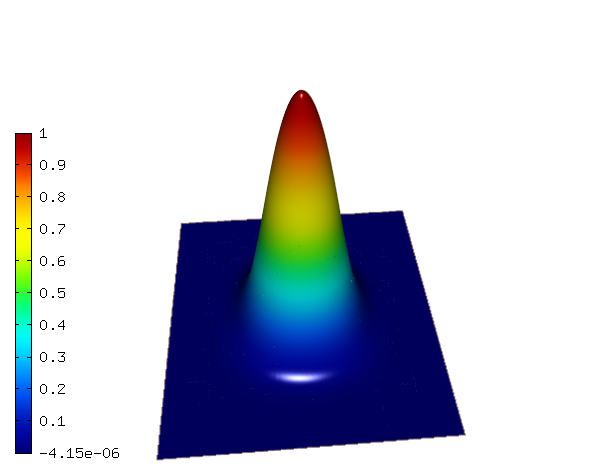
\includegraphics[height=5.5cm]{nist/nist-1/solution.png}
\caption{The solution to NIST-1 benchmark problem.}
\label{fig:sln-nist01}
\end{figure}
\noindent
The goal of the benchmark is to reach a relative error below
$10^{-2}$~\% in the $H^1$-norm with as few degrees of freedom (DOF)
as possible.
We begin with adaptive $hp$-FEM with possibly anisotropic refinements (adaptivity mode
HP\_ANISO in {\sc Hermes}). The initial mesh is shown in Fig. \ref{fig:nist-1-hp-aniso} (left).
In a few adaptivity steps, the polynomial degree of this element is increased
anisotropically.
The resulting mesh with 769 DOF is shown in Fig. \ref{fig:nist-1-hp-aniso} (right).

\begin{figure}[!ht]
\centering
\includegraphics[height=5cm]{nist/nist-1/mesh_hp_aniso_init.png}\ \
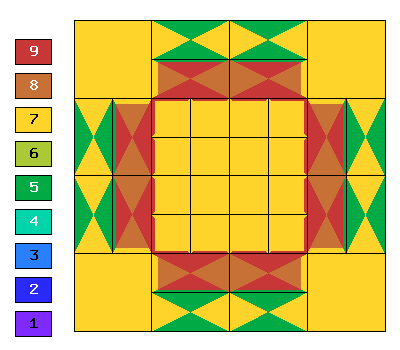
\includegraphics[height=5cm]{nist/nist-1/mesh_hp_aniso.png}
\vspace{-2mm}
\caption{Initial mesh (left) and final mesh (right) for $hp$-FEM with anisotropic refinements.}
\label{fig:nist-1-hp-aniso}
\end{figure}

The final relative error estimate in $H^1$-norm was 3.91108e-03 \%,
and it was identical to the exact error in all printed digits.
We also solved this benchmark with adaptive $h$-FEM
with linear (left) and quadratic (right)
elements, with anisotropic refinements enabled.
Final meshes for the $h$-FEM computations are shown
in Fig. \ref{fig:nist-1-h-aniso}.

\begin{figure}[!ht]
\centering
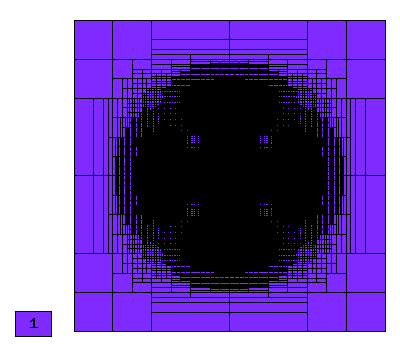
\includegraphics[height=5cm]{nist/nist-1/mesh_h1_aniso.png}\ \
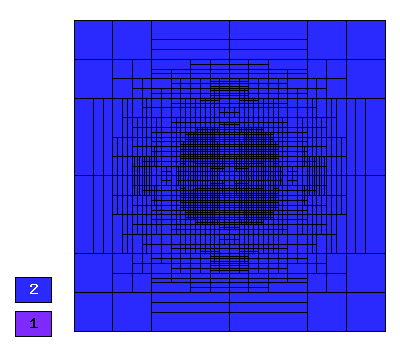
\includegraphics[height=5cm]{nist/nist-1/mesh_h2_aniso.png}
\vspace{-2mm}
\caption{Final mesh for $h$-FEM anisotropic refinements with linear and quadratic elements.}
\label{fig:nist-1-h-aniso}
\end{figure}

Figs. \ref{fig:nist-1-conv} compare all
three approaches to automatic adaptivity  from the point
of view of DOF and CPU convergence.

\begin{figure}[!ht]
\centering
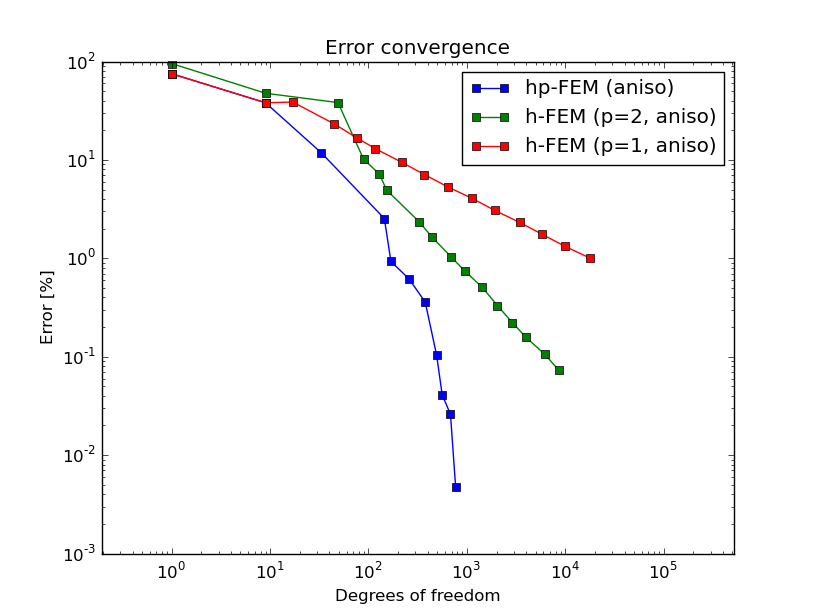
\includegraphics[height=5cm]{nist/nist-1/conv_dof_aniso.png}\ \
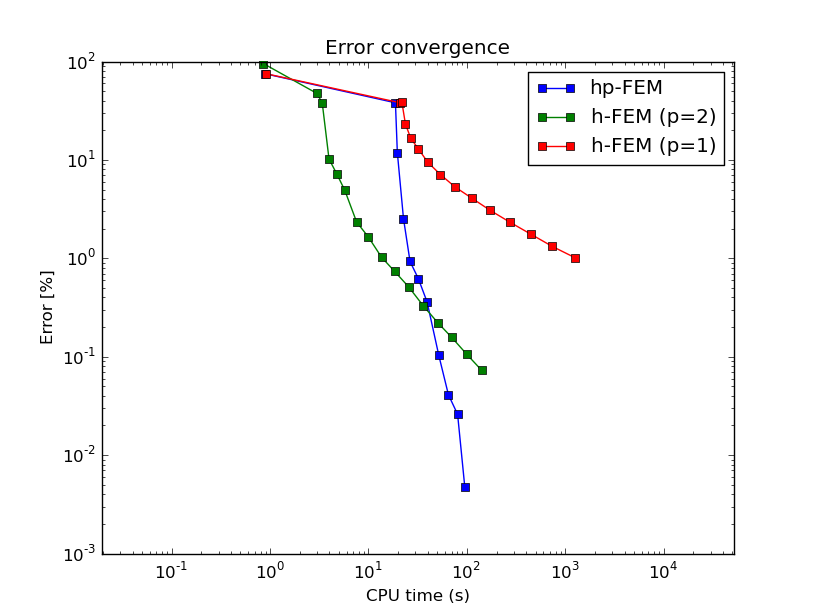
\includegraphics[height=5cm]{nist/nist-1/conv_cpu_aniso.png}
\vspace{-2mm}
\caption{DOF and CPU time convergence graphs.}
\label{fig:nist-1-conv}
\end{figure}

\section{Benchmark NIST-2 "Reentrant Corner"}
\label{sec:bench-2}

This is a standard benchmark for adaptive FEM algorithms.
A reentrant corner is nothing more than an internal or inside corner.
It is a very frequent problem and it can cause the error of the solution
calculated by an adaptive method to converge very slowly or not to converge at all.
The exact solution of this problem is smooth but it contains
singular gradient in the reentrant corner.
The equation solved is the Laplace's equation.

\begin{equation} \label{laplace}
-\Delta u = 0,
\end{equation}

in the domain $\Omega = (-1, 1)^2$, with a unit square
section removed from the bottom part of the positive $x$ axis.
Equation (\ref{laplace}) equipped with Dirichlet
boundary conditions given by the exact solution:

\begin{equation}\label{exact-nist-2}
u(x, y) = r^{\alpha}\sin(\alpha \theta),
\end{equation}

where $\alpha = \pi / \omega$, $r = \sqrt{x^2+y^2}$,
and $\theta = tan^{-1}(y/x)$. Here $\omega $ determines
the angle of the reentrant corner.
The solution of NIST-2 with $\omega = 3 \pi / 2$
is shown in Fig. \ref{fig:sln-nist02}.

\begin{figure}[!ht]
\centering
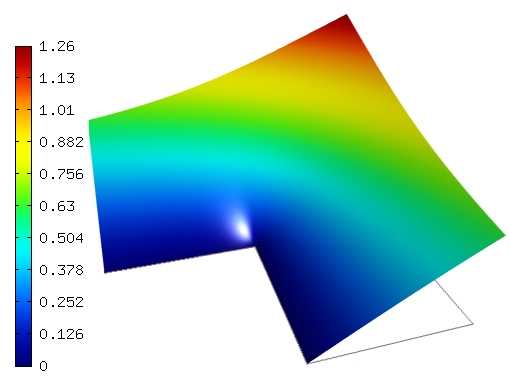
\includegraphics[height=5cm]{nist/nist-2/solution.png}
\caption{The solution to NIST-2 benchmark problem.}
\label{fig:sln-nist02}
\end{figure}

The goal of the benchmark is to reach a relative error below
$10^{-1}$~\% in the $H^1$-norm with as few DOFs as possible.
We begin with adaptive $hp$-FEM,
the initial mesh is shown in Fig. \ref{fig:nist-2-hp-aniso} (left).
After 13 adaptivity steps, the resulting mesh with 622 DOF is shown
in Fig. \ref{fig:nist-2-hp-aniso} (right).

\begin{figure}[!ht]
\centering
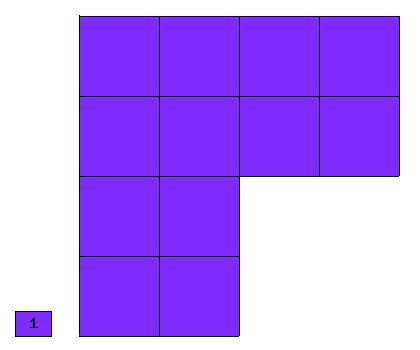
\includegraphics[height=5cm]{nist/nist-2/mesh_hp_aniso_init.png}\ \
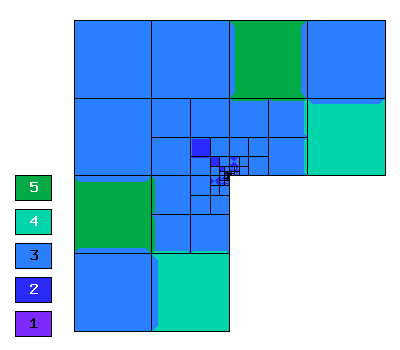
\includegraphics[height=5cm]{nist/nist-2/mesh_hp_aniso.png}
%\vspace{-2mm}
\caption{Initial mesh (left) and final mesh (right) for $hp$-FEM with anisotropic refinements.}
\label{fig:nist-2-hp-aniso}
\end{figure}

The final relative error estimate in $H^1$-norm was 8.15289e-02 \%,
and it was identical to the exact error in all printed digits.
We also solved this benchmark with adaptive $h$-FEM
with linear (left) and quadratic (right)
elements, with anisotropic refinements enabled.
Final meshes for the $h$-FEM computations are shown
in Fig. \ref{fig:nist-2-h-aniso}.

\begin{figure}[!ht]
\centering
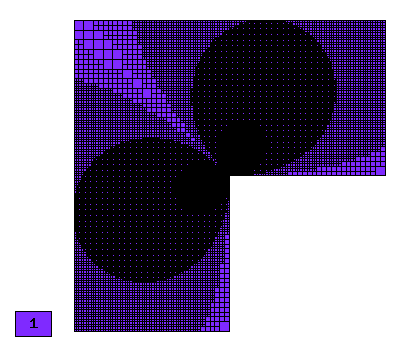
\includegraphics[height=5cm]{nist/nist-2/mesh_h1_aniso.png}\ \
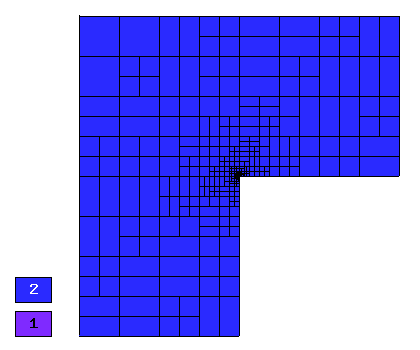
\includegraphics[height=5cm]{nist/nist-2/mesh_h2_aniso.png}
%\vspace{-2mm}
\caption{Final mesh for $h$-FEM anisotropic refinements with linear and quadratic elements.}
\label{fig:nist-2-h-aniso}
\end{figure}

Finally, Figs. \ref{fig:nist-2-conv} compare all
three approaches to automatic adaptivity from the point
of view of DOF and CPU convergence.

\begin{figure}[!ht]
\centering
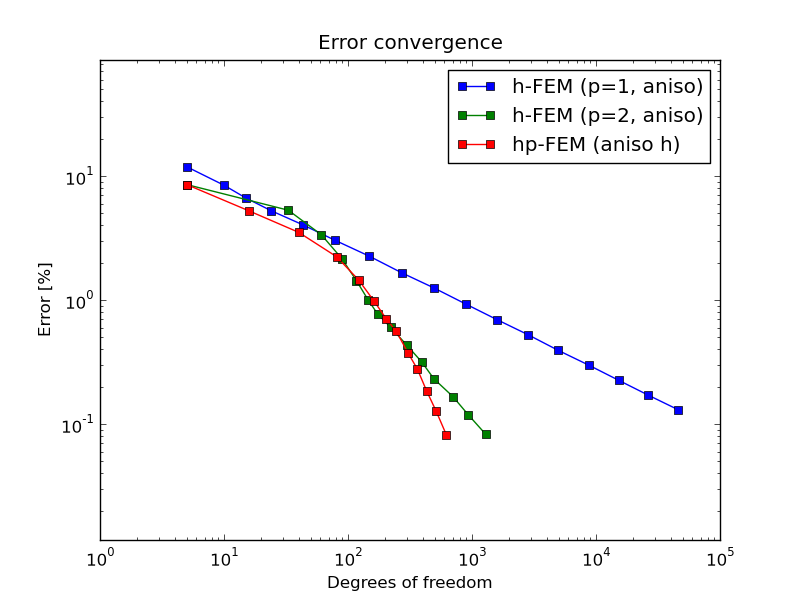
\includegraphics[height=5cm]{nist/nist-2/conv_dof_aniso.png}\ \
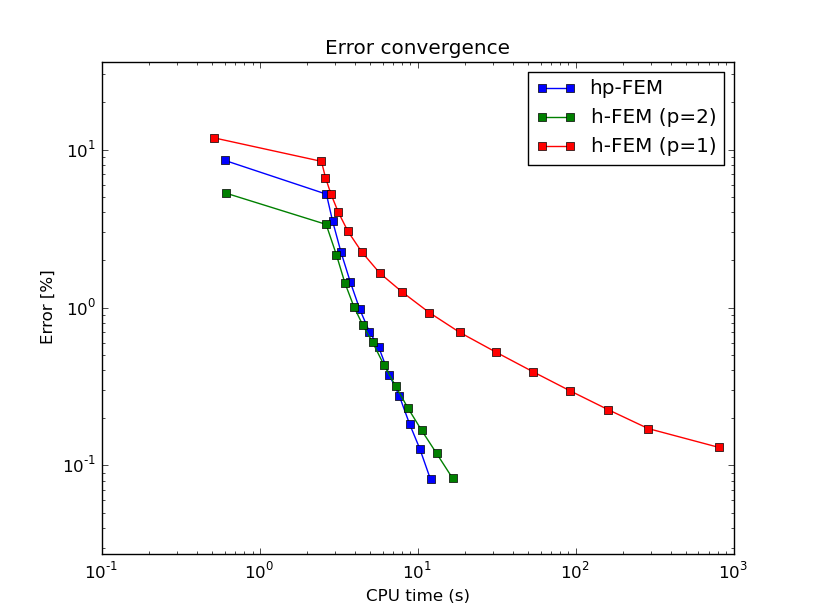
\includegraphics[height=5cm]{nist/nist-2/conv_cpu_aniso.png}
\caption{DOF and CPU time convergence graphs.}
\label{fig:nist-2-conv}
\end{figure}


\section{Benchmark NIST-3 "Linear Elasticity"}
\label{sec:bench-3}

This is a system of two coupled equations with a mixed
derivative for linear elasticity in the coupling term.

\begin{equation} \label{crack-u}
-E \frac{1-\nu^2}{1-2\nu} \frac{\partial^{2} u}{\partial x^{2}} - E\frac{1-\nu^2}{2-2 \nu} \frac{\partial^{2} u}{\partial y^{2}}
-E \frac{1-\nu^2}{(1-2\nu)(2-2\nu)} \frac{\partial^{2} v}{\partial x \partial y} = F_{x}
\end{equation}
\begin{equation} \label{crack-v}
-E \frac{1-\nu^2}{2-2\nu} \frac{\partial^{2} v}{\partial x^{2}} - E\frac{1-\nu^2}{1-2\nu} \frac{\partial^{2} v}{\partial y^{2}}
-E \frac{1-\nu^2}{(1-2\nu)(2-2\nu)} \frac{\partial^{2} u}{\partial x \partial y} = F_{y},
\end{equation}
where $F_{x} = F_{y} = 0$, $u$ and $v$ are the
$x$ and $y$ displacements, $E$ is Young's Modulus,
and $\nu$ is Poisson's ratio.

The domain is $\Omega = (0, 1)^2$, equipped with Dirichlet
boundary conditions given by the exact solution.

The exact solution:
\begin{equation}\label{exact-nist-3-u-1}
u(x, y) = \frac{1}{2G} r^{\lambda}[(k - Q(\lambda + 1))cos(\lambda \theta) - \lambda cos((\lambda - 2) \theta)]
\end{equation}
\begin{equation}\label{exact-nist-3-v-1}
v(x, y) = \frac{1}{2G} r^{\lambda}[(k + Q(\lambda + 1))sin(\lambda \theta) + \lambda sin((\lambda - 2) \theta)]
\end{equation}
here $\lambda = 0.5444837367825$, $Q = 0.5430755788367$,
$k = 3 - 4 \nu$ and $G = E / (2(1 + \nu))$.

The solution of NIST-3 is shown in Fig. \ref{fig:sln-nist03}.

\begin{figure}[!ht]
\centering
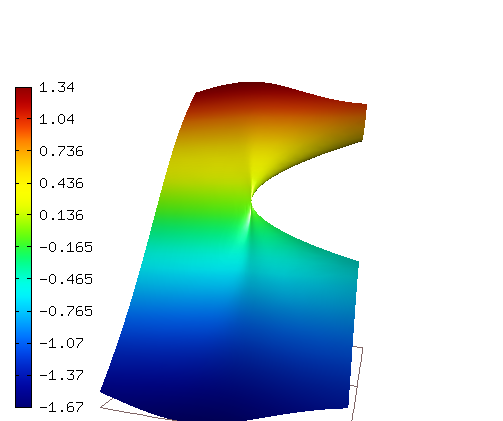
\includegraphics[height=50mm]{nist/nist-3/solution-u.png}\ \
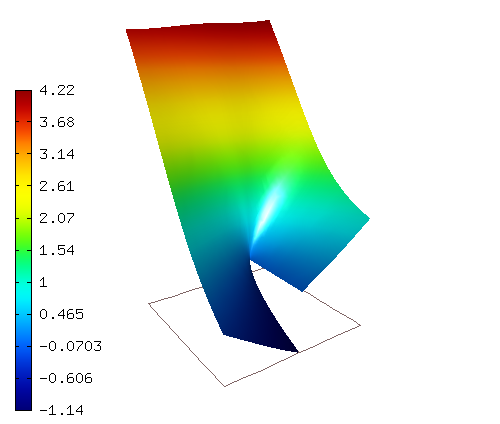
\includegraphics[height=50mm]{nist/nist-3/solution-v.png}
\vspace{-2mm}
\caption{The $u$ and $v$ component to NIST-3 benchmark problem.}
\label{fig:sln-nist03}
\end{figure}

\section{Benchmark NIST-4 "Peak"}
\label{sec:bench-4}

This problem has an exponential peak in the interior of the domain.
The equation solved in this benchmark problem is the Poisson's equation.

\begin{equation} \label{poisson-peak}
-\Delta u = f,
\end{equation}
in the domain $\Omega = (0, 1)^2$, equipped with Dirichlet
boundary conditions given by the exact solution.

The exact solution:
\begin{equation}\label{exact-nist-4}
u(x,y) = e^{-\alpha ((x - x_{loc})^{2} + (y - y_{loc})^{2})},
\end{equation}
where $(x_{loc}, y_{loc})$ is the location of the peak, and $\alpha$ determines the strength of the peak.
The right-hand side $f$ is calculated by inserting (\ref{exact-nist-4}) into (\ref{poisson-peak}).
The solution of NIST-4 with $\alpha = 1000$, $(x_{loc}, y_{loc}) = (0.5, 0.5)$ is shown in Fig. \ref{fig:sln-nist04}.

\begin{figure}[!ht]
\centering
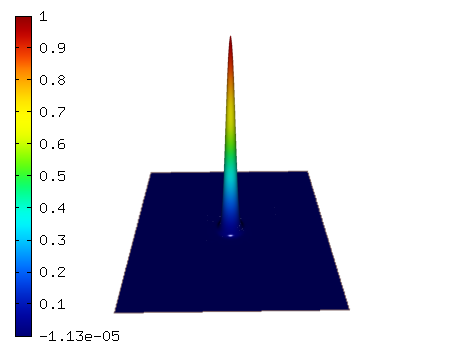
\includegraphics[height=6cm]{nist/nist-4/solution.png}
\caption{The solution to NIST-4 benchmark problem.}
\label{fig:sln-nist04}
\end{figure}

\section{Benchmark NIST-5 "Battery"}
\label{sec:bench-5}

This is a heat conduction problem in a nonhomogeneous material. It comes with an anisotropic solution and
multiple singularities. The solution has multiple point singularities in the interior of the domain.
The equation is given below

\begin{equation} \label{heat-conduction}
-\frac{\partial }{\partial x}\left(p(x, y)\frac{\partial u}{\partial x}\right)
-\frac{\partial }{\partial y}\left(q(x, y)\frac{\partial u}{\partial y}\right) = f
\end{equation}
in the domain $\Omega = (0, 8.4) \times (0, 24)$, equipped with
a zero Neumann boundary condition on left edge, Natural boundary conditions on the rest of the boundary.

\begin{equation}
p(x, y)\frac{\partial u}{\partial x}\nu_1 + q(x, y)\frac{\partial u}{\partial y}\nu_2 = g_{left}(x, y) \ \mbox{on} \  \Gamma_{left}
\end{equation}

\begin{equation}
p(x, y)\frac{\partial u}{\partial x}\nu_1 + q(x, y)\frac{\partial u}{\partial y}\nu_2 + c(x, y)u = g_{right}(x, y) \ \mbox{on} \ \Gamma_{right}
\end{equation}

\begin{equation}
p(x, y)\frac{\partial u}{\partial x}\nu_1 + q(x, y)\frac{\partial u}{\partial y}\nu_2 + c(x, y)u = g_{top}(x, y) \ \mbox{on} \ \Gamma_{top}
\end{equation}

\begin{equation}
p(x, y)\frac{\partial u}{\partial x}\nu_1 + q(x, y)\frac{\partial u}{\partial y}\nu_2 + c(x, y)u = g_{bottom}(x, y) \ \mbox{on} \ \Gamma_{bottom}
\end{equation}
where $p(x, y)$, $q(x, y)$, $c(x, y)$, $g(x, y)$
and the right hand side $f$ are constant coefficient
functions in different materials.

The solution of NIST-5 is shown in Fig. \ref{fig:sln-nist05}.
\begin{figure}[!ht]
\centering
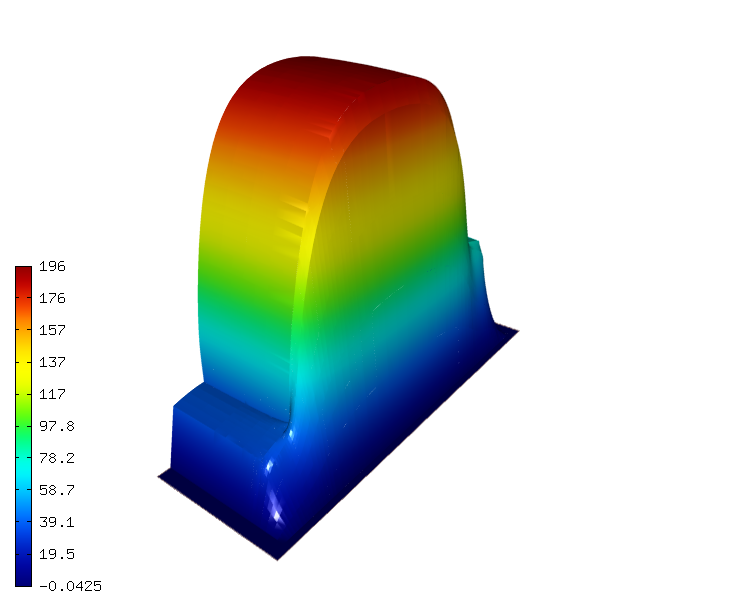
\includegraphics[height=40mm]{nist/nist-5/solution-3d.png}
\caption{The solution to NIST-5 benchmark problem.}
\label{fig:sln-nist05}
\end{figure}

\section{Benchmark NIST-6 "Boundary Layer"}
\label{sec:bench-6}

Solution of this problem has a boundary layer along the right and top sides of the domain.
It is a convection-diffusion equation with first order terms.

\begin{equation} \label{boundary-layer}
-\epsilon \nabla^{2} u + 2\frac{\partial u}{\partial x} + \frac{\partial u}{\partial y}= f
\end{equation}
in the domain $\Omega = (-1, 1)^2$, equipped with Dirichlet boundary condition
given by the exact solution.

The exact solution:
\begin{equation}\label{exact-nist-6}
u(x,y) = (1 - e^{-(1 - x) / \epsilon})(1 - e^{-(1 - y) / \epsilon})cos(\pi (x + y)),
\end{equation}
where $\epsilon$ determines the strength of the boundary layer.
The right-hand side $f$ is calculated by inserting (\ref{exact-nist-6}) into (\ref{boundary-layer}).
The solution of NIST-6 with $\epsilon = 10^{-1}$ is shown in Fig. \ref{fig:sln-nist06}.

\begin{figure}[!ht]
\centering
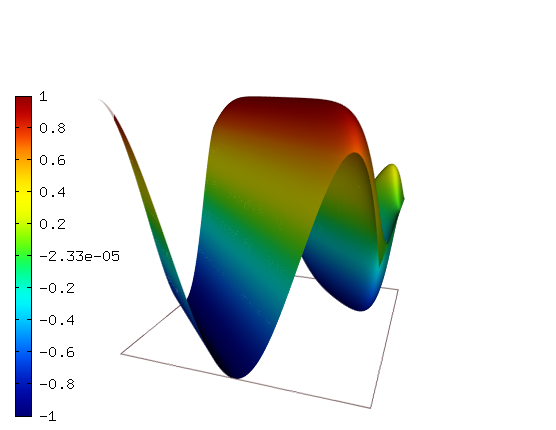
\includegraphics[height=5cm]{nist/nist-6/solution.png}
\caption{The solution to NIST-6 benchmark problem.}
\label{fig:sln-nist06}
\end{figure}

The goal of the benchmark is to reach a relative error below
$10^{-3}$~\% in the $H^1$-norm with as few DOFs as possible.
We begin with adaptive $hp$-FEM with possibly anisotropic refinements.
The initial mesh is shown in Fig. \ref{fig:nist-6-hp-aniso} (left).
In a few adaptivity steps, the polynomial degree of this domain is increased
anisotropically.
The resulting mesh with 591 DOF is shown in Fig. \ref{fig:nist-6-hp-aniso} (right).

\begin{figure}[!ht]
\centering
\includegraphics[height=5cm]{nist/nist-6/mesh_hp_aniso_init.png}\ \
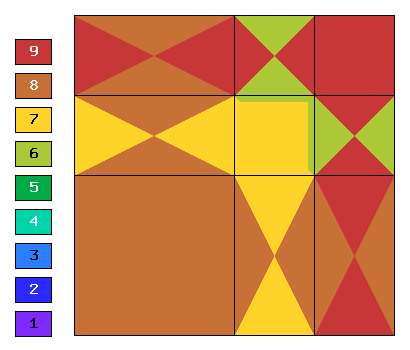
\includegraphics[height=5cm]{nist/nist-6/mesh_hp_aniso.png}
\vspace{-2mm}
\caption{Initial mesh (left) and final mesh (right) for $hp$-FEM with anisotropic refinements.}
\label{fig:nist-6-hp-aniso}
\end{figure}

The final relative error estimate in $H^1$-norm was 6.23458e-04 \%,
and it was identical to the exact error in all printed digits.
We also solved this benchmark with adaptive $h$-FEM
with linear (left) and quadratic (right)
elements, with anisotropic refinements enabled.
Final meshes for the $h$-FEM computations are shown
in Fig. \ref{fig:nist-6-h-aniso}.

\begin{figure}[!ht]
\centering
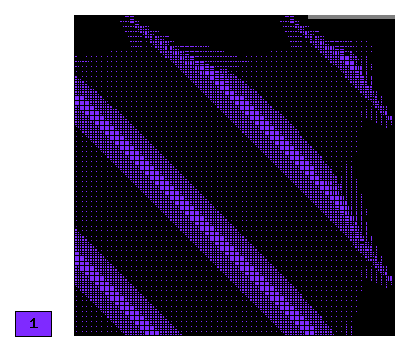
\includegraphics[height=5cm]{nist/nist-6/mesh_h1_aniso.png}\ \
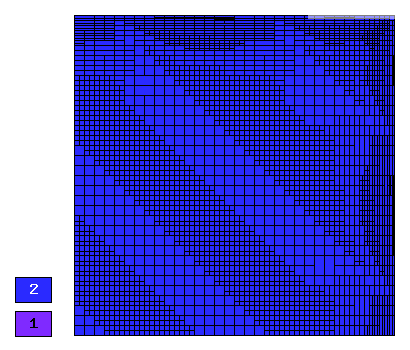
\includegraphics[height=5cm]{nist/nist-6/mesh_h2_aniso.png}
\vspace{-2mm}
\caption{Final mesh for $h$-FEM anisotropic refinements with linear and quadratic elements.}
\label{fig:nist-6-h-aniso}
\end{figure}

Figs. \ref{fig:nist-6-conv} compare all
three approaches to automatic adaptivity from the point
of view of DOF and CPU convergence.

\begin{figure}[!ht]
\centering
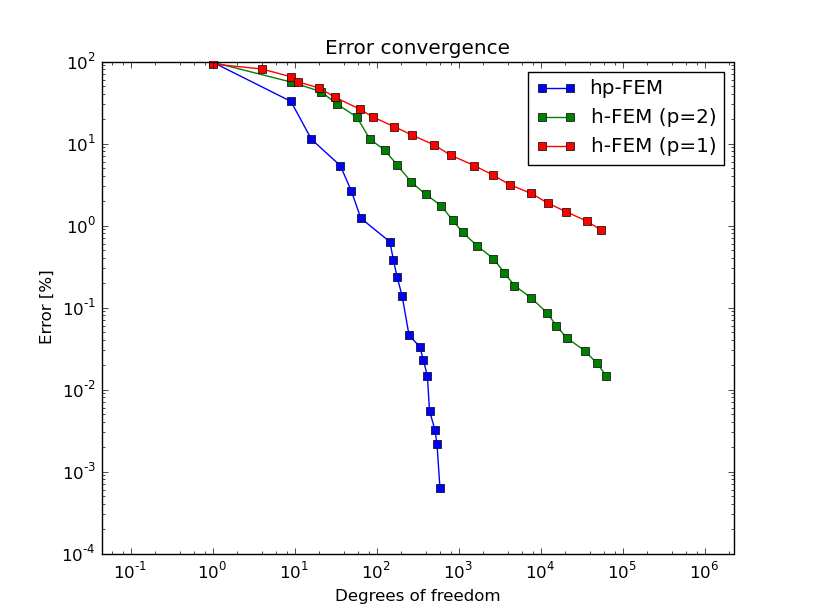
\includegraphics[height=5cm]{nist/nist-6/conv_dof_aniso.png}\ \
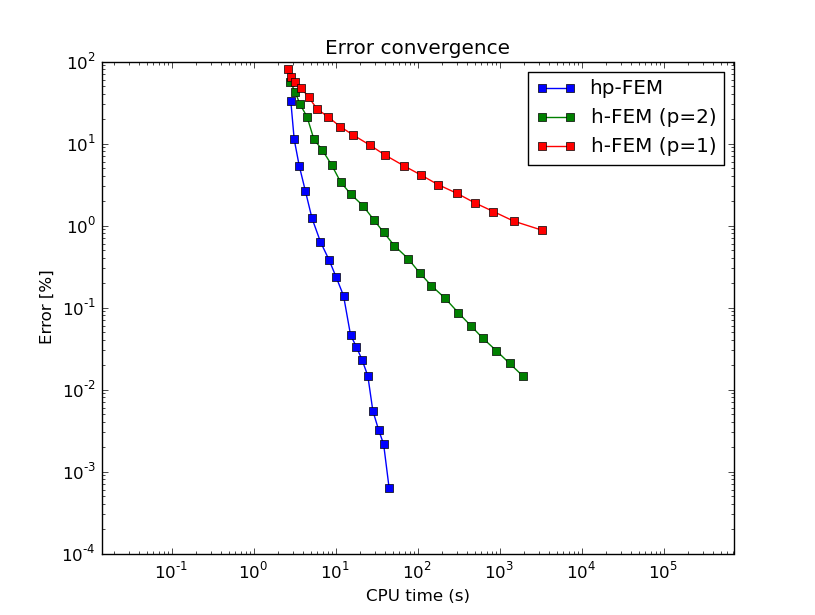
\includegraphics[height=5cm]{nist/nist-6/conv_cpu_aniso.png}
\caption{DOF and CPU time convergence graphs.}
\label{fig:nist-6-conv}
\end{figure}


\section{Benchmark NIST-7 "Boundary Line Singularity"}
\label{sec:bench-7}

This is a singularity problem with a solution that is singular along the left boundary.
The equation of this problem is Poisson equation

\begin{equation} \label{boundary-line-singularity}
-\Delta u = f
\end{equation}
in the domain $\Omega = (0, 1)^2$, equipped with Dirichlet boundary conditions
given by the exact solution.

The exact solution
\begin{equation}\label{exact-nist-7}
u(x,y) = x^{\alpha}
\end{equation}
where $\alpha \geq 0.5$ determines the strength of the singularity.
The right-hand side $f$ is calculated by inserting (\ref{exact-nist-7}) into (\ref{boundary-line-singularity}).
The solution of NIST-7 with $\alpha = 0.6$ is shown in Fig. \ref{fig:sln-nist07}.

\begin{figure}[!ht]
\centering
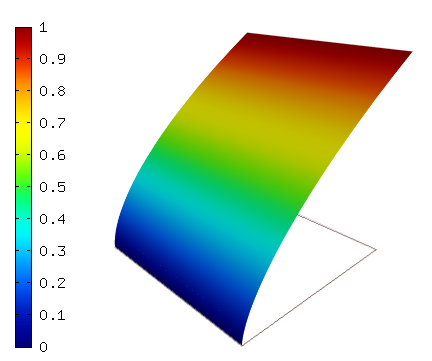
\includegraphics[height=6cm]{nist/nist-7/solution.png}
\caption{The solution to NIST-7 benchmark problem.}
\label{fig:sln-nist07}
\end{figure}

\section{Benchmark NIST-8 "Oscillatory"}
\label{sec:bench-8}

This is a wave function that satisfies the Schr\"{o}dinger's equation model of two
interacting atoms, highly oscillatory near the origin.
The equation solved in this problem is the Helmholtz equation.

\begin{equation} \label{oscillatory}
-\nabla^{2} u - \frac{1}{(\alpha + r)^{4}} u = f
\end{equation}
in the domain $\Omega = (0, 1)^2$, equipped with Dirichlet boundary conditions
given by the exact solution. The exact solution is
$u(x,y) = sin(\frac{1}{\alpha + r})$,
where $r = \sqrt{x^{2} + y^{2}}$, $\alpha = 1 / N \pi$ determines the number of oscillations.
The right-hand side $f$ is calculated by inserting exact solution into (\ref{oscillatory}).
The solution of NIST-8 with $\alpha = 1 / 10 \pi$ is shown in Fig. \ref{fig:sln-nist08}.

\begin{figure}[!ht]
\centering
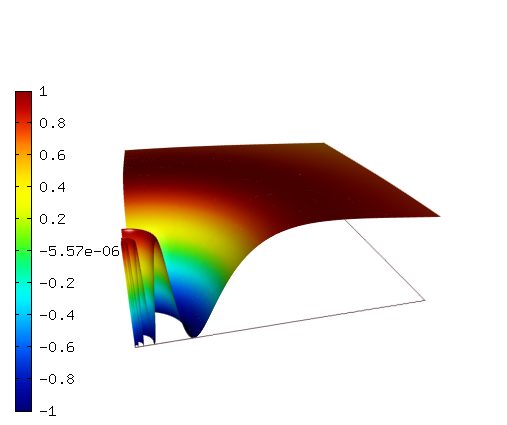
\includegraphics[height=5cm]{nist/nist-8/solution.png}
\caption{The solution to NIST-8 benchmark problem.}
\label{fig:sln-nist08}
\end{figure}

\begin{figure}[!ht]
\centering
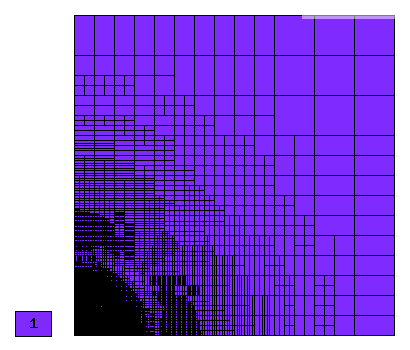
\includegraphics[height=3.7cm]{nist/nist-8/mesh_h1_aniso.png}
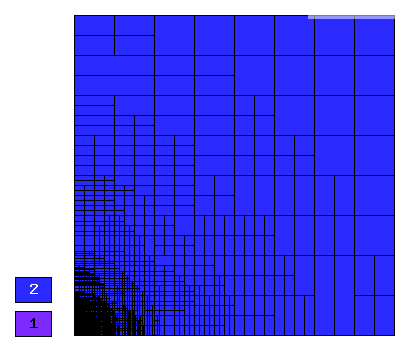
\includegraphics[height=3.7cm]{nist/nist-8/mesh_h2_aniso.png}
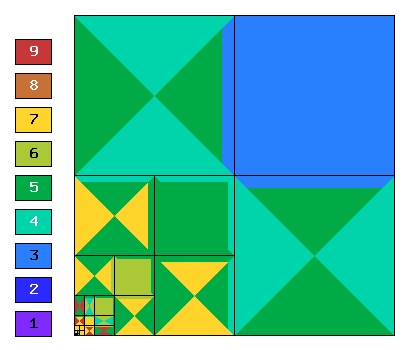
\includegraphics[height=3.7cm]{nist/nist-8/mesh_hp_aniso.png}
\caption{
Final mesh (left) with 55731 DOF and the resulting
relative error estimate in $H^1$-norm of 1.24198 \% for $h$-FEM with linear elements.
Final mesh (middle) with 3413 DOF and the resulting
relative error estimate in $H^1$-norm of 6.64833e-01 1.49585 \% for $h$-FEM with quadratic elements.
Final mesh (right) with 1160 DOF and the resulting
relative error estimate in $H^1$-norm of 9.09848e-02 \% for $hp$-FEM with anisotropic refinements.}
\label{fig:nist-8-hp-aniso}
\end{figure}

%\begin{figure}[!ht]
%\centering
%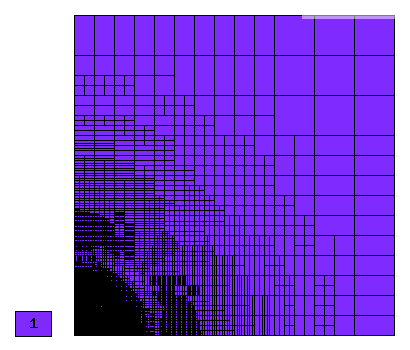
\includegraphics[height=5cm]{nist/nist-8/mesh_h1_aniso.png}\ \
%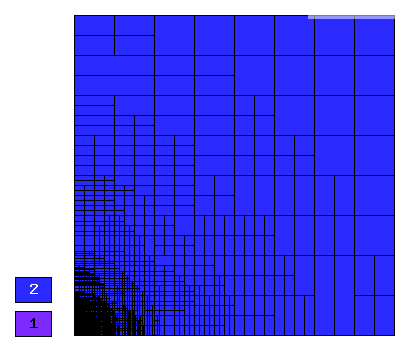
\includegraphics[height=5cm]{nist/nist-8/mesh_h2_aniso.png}
%\caption{Final mesh for $h$-FEM with linear and quadratic elements.}
%\label{fig:nist-8-h-aniso}
%\end{figure}

Figs. \ref{fig:nist-8-conv} compare all
three approaches to automatic adaptivity from the point
of view of DOF and CPU convergence.

\begin{figure}[!ht]
\centering
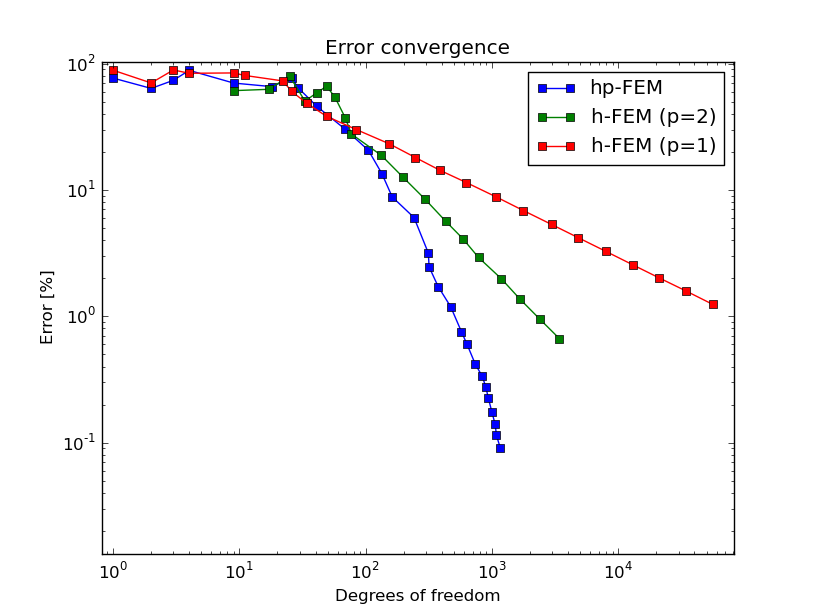
\includegraphics[height=5cm]{nist/nist-8/conv_dof_aniso.png}\ \
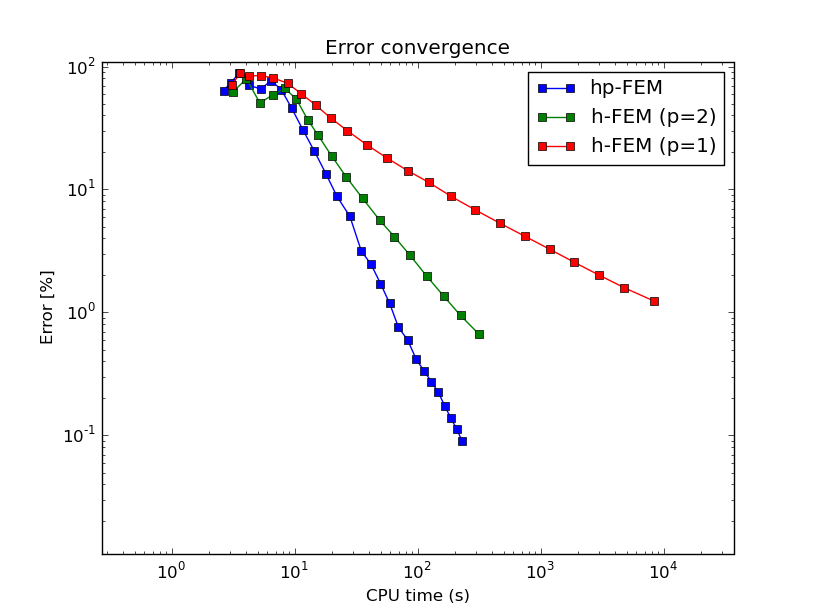
\includegraphics[height=5cm]{nist/nist-8/conv_cpu_aniso.png}
\caption{DOF and CPU time convergence graphs.}
\label{fig:nist-8-conv}
\end{figure}


\section{Benchmark NIST-9 "Wave Front"}
\label{sec:bench-9}

This is a commonly used example for testing the performance of
adaptive refinement algorithms on the wave front and the singularity \cite{mitchell-1, mitchell-2}.
The solution has a sharp circular wave front in the interior of the
domain, with a singularity at the center of the circle.
The equation solved is the Poisson's equation.

\begin{equation} \label{wave-front}
-\Delta u = f
\end{equation}

in the domain $\Omega = (0, 1)^2$, equipped with Dirichlet boundary conditions
given by the exact solution. The exact solution:

\begin{equation}\label{exact-nist-9}
u(x, y) = tan^{-1}(\alpha (r - r_{0}))
\end{equation}

where $r = \sqrt{(x - x_{loc})^{2} + (y - y_{loc})^{2}}$.
Here $(x_{loc}, y_{loc})$ is the center of the circular wave front,
$r_{0}$ is the distance from the wave front to the center of the circle,
and $\alpha$ gives the steepness of the wave front.
The right-hand side $f$ is calculated by inserting (\ref{exact-nist-9}) into (\ref{wave-front}).
The solution of NIST-9 with $\alpha = 50$, $(x_{loc}, y_{loc}) = (0.5, 0.5)$,
$r_{0} = 0.25$ is shown in Fig. \ref{fig:sln-nist09}.

\begin{figure}[!ht]
\centering
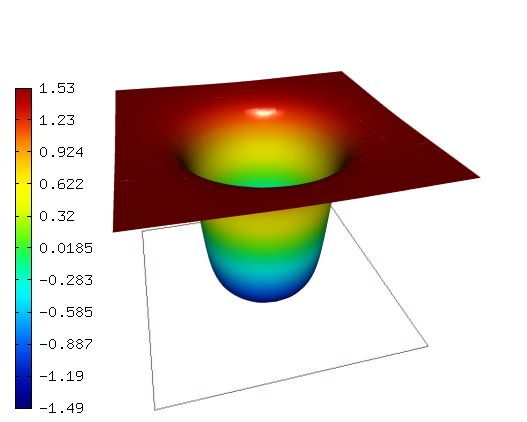
\includegraphics[height=6cm]{nist/nist-9/solution.png}
\caption{The solution to NIST-9 benchmark problem.}
\label{fig:sln-nist09}
\end{figure}

The goal of the benchmark is to reach a relative error below
$10^{-1}$~\% in the $H^1$-norm with as few DOFs as possible.
We begin with adaptive $hp$-FEM,
the initial mesh is shown in Fig. \ref{fig:nist-9-hp-aniso} (left).
After 13 adaptivity steps, the resulting mesh with 1465 DOF is shown
in Fig. \ref{fig:nist-9-hp-aniso} (right).

\begin{figure}[!ht]
\centering
\includegraphics[height=5cm]{nist/nist-9/mesh_hp_aniso_init.png}\ \
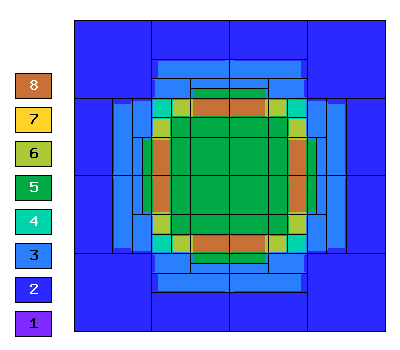
\includegraphics[height=5cm]{nist/nist-9/mesh_hp_aniso.png}
\caption{Initial mesh (left) and final mesh (right) for $hp$-FEM with anisotropic refinements.}
\label{fig:nist-9-hp-aniso}
\end{figure}

The final relative error estimate in $H^1$-norm was 8.67667e-01 \%,
and it was identical to the exact error in all printed digits.
We also solved this benchmark with adaptive $h$-FEM
with linear (left) and quadratic (right)
elements, with anisotropic refinements enabled.
Final meshes for the $h$-FEM computations are shown
in Fig. \ref{fig:nist-9-h-aniso}.

\begin{figure}[!ht]
\centering
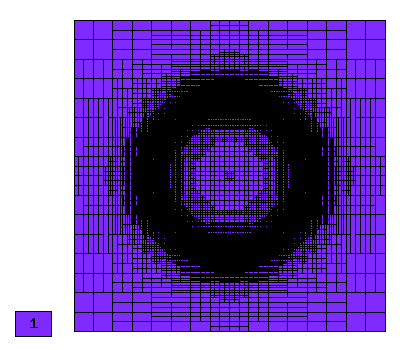
\includegraphics[height=5cm]{nist/nist-9/mesh_h1_aniso.png}\ \
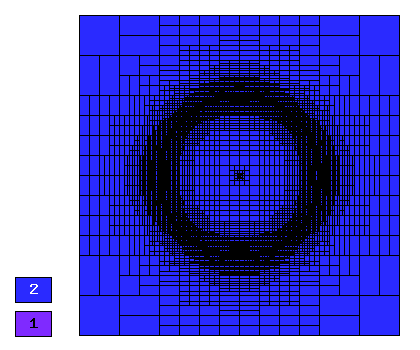
\includegraphics[height=5cm]{nist/nist-9/mesh_h2_aniso.png}
\caption{Final mesh for $h$-FEM anisotropic refinements with linear and quadratic elements.}
\label{fig:nist-9-h-aniso}
\end{figure}

Finally, Figs. \ref{fig:nist-9-conv} compare all
three approaches to automatic adaptivity from the point
of view of DOF and CPU convergence.

\begin{figure}[!ht]
\centering
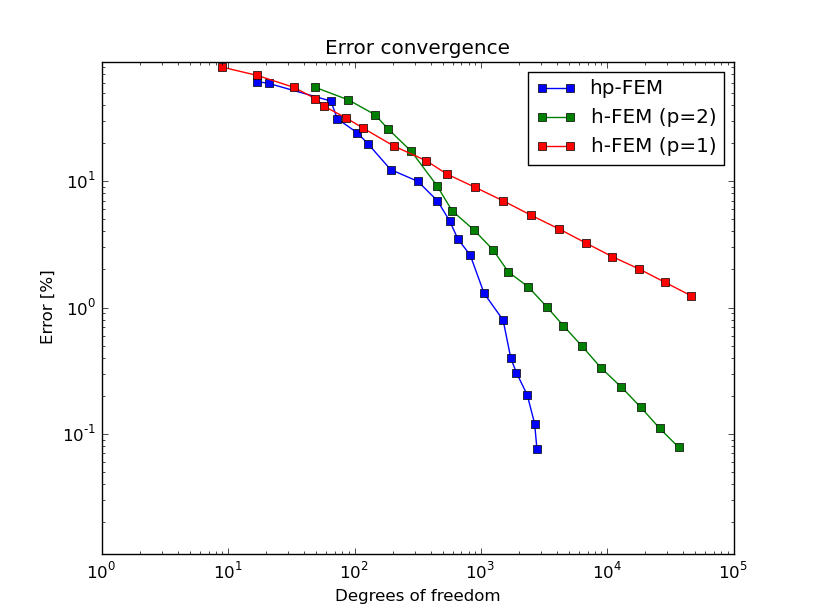
\includegraphics[height=5cm]{nist/nist-9/conv_dof_aniso.png}\ \
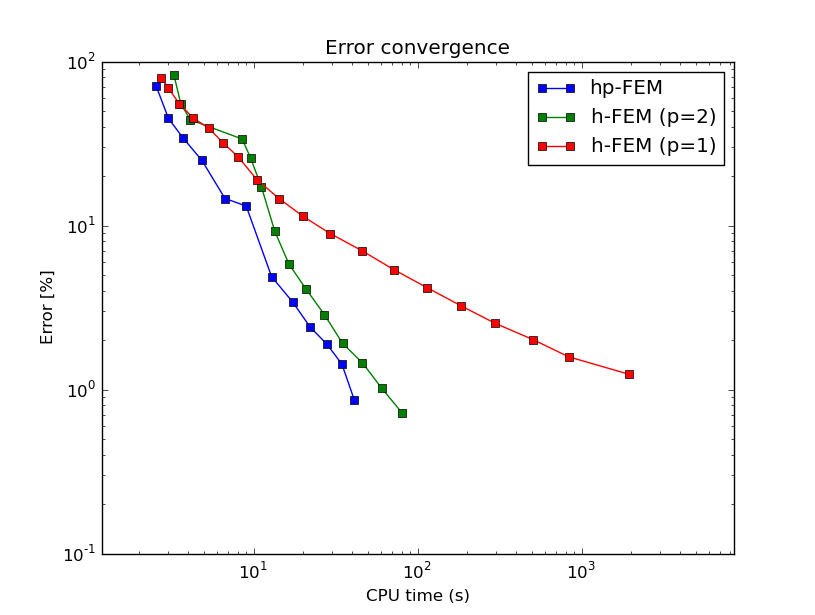
\includegraphics[height=5cm]{nist/nist-9/conv_cpu_aniso.png}
\caption{DOF and CPU time convergence graphs.}
\label{fig:nist-9-conv}
\end{figure}


\section{Benchmark NIST-10 "Interior Line Singularity"}
\label{sec:bench-10}

This is another example with anisotropic solution that is suitable for testing
anisotropic element refinements. The equation solved is the Poisson's equation.
(Note: we need more description...)

\begin{equation} \label{interior}
-\Delta u = f
\end{equation}

in the domain $\Omega = (-1, 1)^2$, equipped with a zero
Neumann boundary condition on left edge, Dirichlet boundary 
conditions given by the exact solution on the rest of the boundary.
The exact solution:

\begin{equation}\label{exact-nist-10}
\left\{
\begin{array}{l}
\displaystyle
u(x,y) = \cos(Ky)\ \ \ \mbox{for}\ x \le 0 \\
u(x,y) = \cos(Ky) + x^{\alpha}\ \ \ \mbox{for}\ x > 0
\end{array}
\right.
\end{equation}

where $K$ and $\alpha$ are real constants.
The right-hand side $f$ is calculated by inserting
(\ref{exact-nist-10}) into (\ref{interior}).
The solution of NIST-10 with $K = \pi/2$ and
$\alpha = 2.01$ is shown in Fig. \ref{fig:sln-nist10}.

\begin{figure}[!ht]
\centering
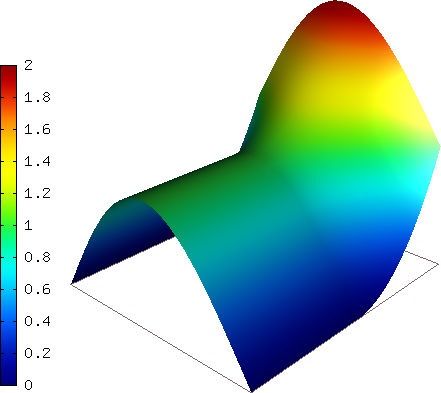
\includegraphics[height=6cm]{nist/nist-10/solution.png}
\caption{The solution to NIST-10 benchmark problem.}
\label{fig:sln-nist10}
\end{figure}

The goal of the benchmark is to reach a relative error below
$10^{-4}$~\% in the $H^1$-norm with as few DOFs as possible.
We begin with adaptive $hp$-FEM, 
the initial mesh is shown in Fig. \ref{fig:nist-10-hp-aniso} (left).
After 14 adaptivity steps, the resulting mesh with 381 DOF is shown 
in Fig. \ref{fig:nist-10-hp-aniso} (right).

\begin{figure}[!ht]
\centering
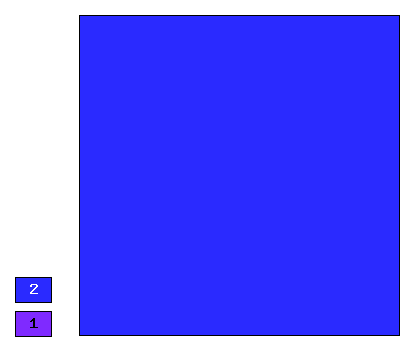
\includegraphics[height=5cm]{nist/nist-10/mesh_hp_aniso_init.png}\ \
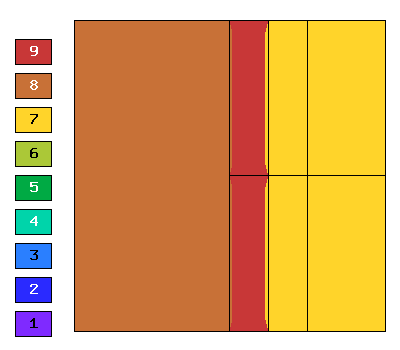
\includegraphics[height=5cm]{nist/nist-10/mesh_hp_aniso.png}
\vspace{-2mm}
\caption{Initial mesh (left) and final mesh (right) for $hp$-FEM with anisotropic refinements.}
\label{fig:nist-10-hp-aniso}
\end{figure}

The final relative error estimate in $H^1$-norm was 8.68994e-05 \%,
and it was identical to the exact error in all printed digits.
We also solved this benchmark with adaptive $h$-FEM
with linear (left) and quadratic (right)
elements, with anisotropic refinements enabled.
Final meshes for the $h$-FEM computations are shown
in Fig. \ref{fig:nist-10-h-aniso}.

\begin{figure}[!ht]
\centering
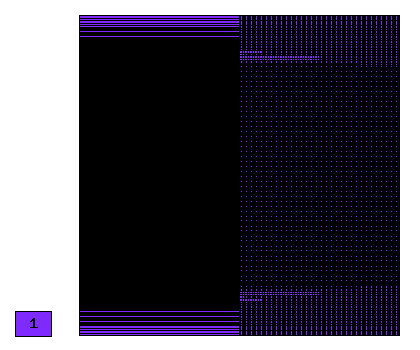
\includegraphics[height=5cm]{nist/nist-10/mesh_h1_aniso.png}\ \
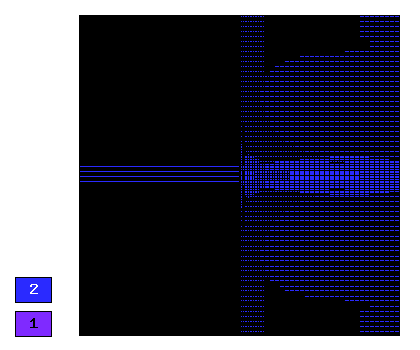
\includegraphics[height=5cm]{nist/nist-10/mesh_h2_aniso.png}
\vspace{-2mm}
\caption{Final mesh for $h$-FEM anisotropic refinements with linear and quadratic elements.}
\label{fig:nist-10-h-aniso}
\end{figure}

Finally, Figs. \ref{fig:nist-10-conv} compare all
three approaches to automatic adaptivity from the point
of view of DOF and CPU convergence.

\begin{figure}[!ht]
\centering
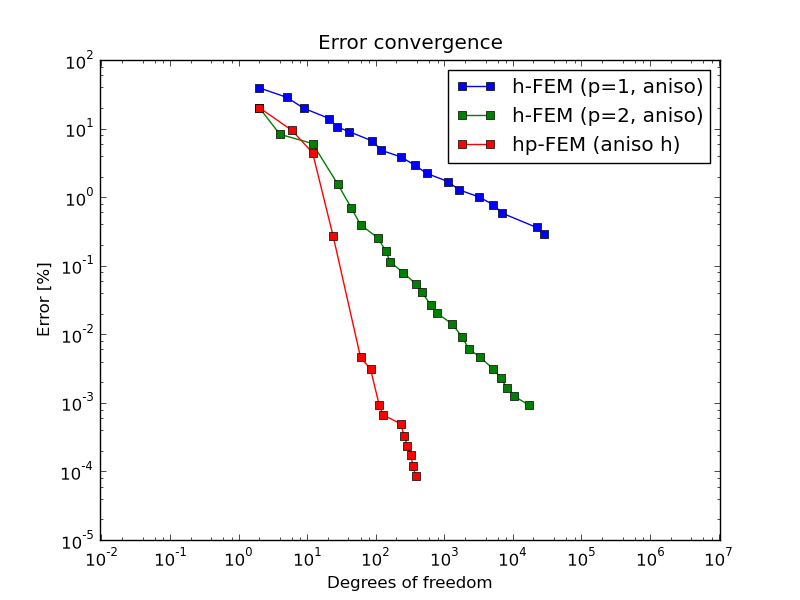
\includegraphics[height=5cm]{nist/nist-10/conv_dof_aniso.png}\ \
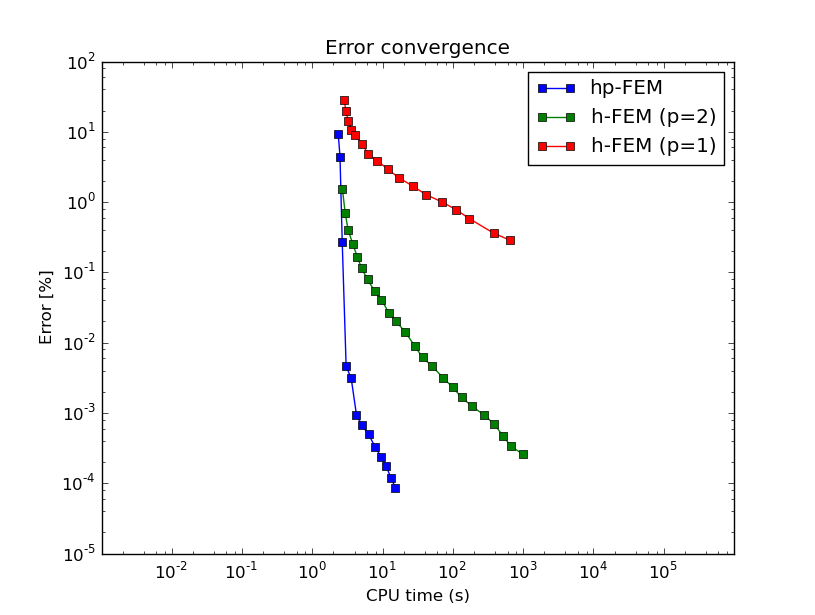
\includegraphics[height=5cm]{nist/nist-10/conv_cpu_aniso.png}
\caption{DOF and CPU time convergence graphs.}
\label{fig:nist-10-conv}
\end{figure}


\section{Benchmark NIST-11 "Intersecting Interfaces"}
\label{sec:bench-11}

This is a Poisson's problem with intersecting interfaces,
dividing the plane into four regions.
The solution to this problem contains a severe
singularity that poses a challenge to adaptive methods.
The equation solved is given by

\begin{equation} \label{intersecting}
-\nabla \cdot (a(x,y) \nabla u) = 0
\end{equation}

where the parameter $a$ is piecewise-constant,
$a(x,y) = 161.4476387975881$ in the first and third quadrants,
and $a(x,y) = 1$ in the remaining two quadrants.
The domain of this problem is $\Omega = (-1, 1)^2$, equipped with
Dirichlet boundary conditions given by the exact solution.
The exact solution is 
$u(x,y) = r^{a_1} \mu (\theta)$,  
where $a_1$ and $\mu (\theta)$ is given in \cite{mitchell-1}.
The right-hand side $f$ is calculated by inserting exact solution into (\ref{intersecting}).
The solution of NIST-11 is shown in Fig. \ref{fig:sln-nist11}.

\begin{figure}[!ht]
\centering
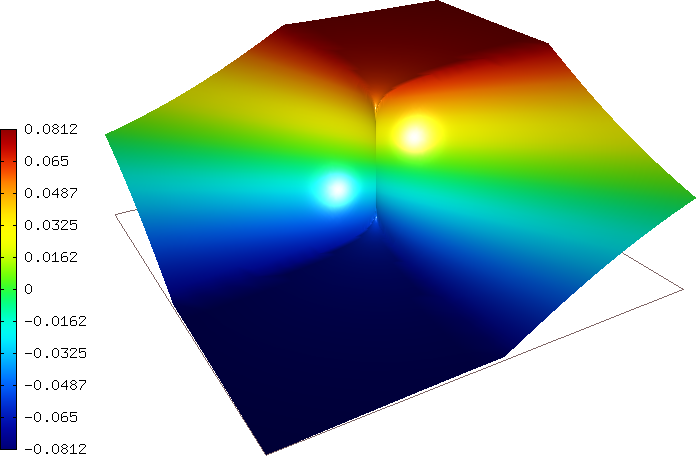
\includegraphics[height=5cm]{nist/nist-11/solution.png}
\caption{The solution to NIST-11 benchmark problem.}
\label{fig:sln-nist11}
\end{figure}

\begin{figure}[!ht]
\centering
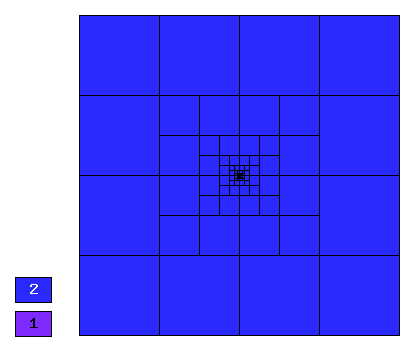
\includegraphics[height=5cm]{nist/nist-11/mesh_hp_aniso_init.png}\ \
\includegraphics[height=5cm]{nist/nist-11/mesh_hp_aniso.png}
\caption{Initial mesh (left) and final mesh (right) with 591 DOF and the resulting relative error estimate in $H^1$-norm of 4.7087e-01 \% for $hp$-FEM with anisotropic refinements.}
\label{fig:nist-11-hp-aniso}
\end{figure}

\begin{figure}[!ht]
\centering
\includegraphics[height=5cm]{nist/nist-11/mesh_h1_aniso.png}\ \
\includegraphics[height=5cm]{nist/nist-11/mesh_h2_aniso.png}
\caption{Final mesh for $h$-FEM with linear and quadratic elements.}
\label{fig:nist-11-h-aniso}
\end{figure}

Figs. \ref{fig:nist-11-conv} compare all
three approaches to automatic adaptivity from the point
of view of DOF and CPU convergence.

\begin{figure}[!ht]
\centering
\includegraphics[height=5cm]{nist/nist-11/conv_dof_aniso.png}\ \
\includegraphics[height=5cm]{nist/nist-11/conv_cpu_aniso.png}
\caption{DOF and CPU time convergence graphs.}
\label{fig:nist-11-conv}
\end{figure}


\section{Benchmark NIST-12 "Multiple Difficulties"}
\label{sec:bench-12}

This problem combines four aspects of benchmarks
seen in previous sections (nist-2, nist-4, nist-6 and nist-9) into one problem.
The wave front intersects the boundary
layer and corner singularity, and the peak is centered on the wave front.
The equation solved is the Poisson's equation.

\begin{equation} \label{multiple}
-\Delta u = f
\end{equation}

in the L-shaped domain, equipped with Dirichlet boundary conditions
given by the exact solution.
The exact solution:

\begin{equation}\label{exact-nist-12}
u(x,y) =  r^{\alpha_{C} }\sin(\alpha_{C} \theta) 
+ e^{-\alpha_{P} ((x - x_{P})^{2} + (y - y_{P})^{2})} 
+ tan^{-1}(\alpha_{W} (r_{W} - r_{0}))
+ e^{-(1 - y) / \epsilon}
\end{equation}

where $\alpha_C = \pi / \omega_C$, $r = \sqrt{x^2+y^2}$
and $\theta = tan^{-1}(y/x)$, here $\omega_C$ determines
the angle of the re-entrant corner.
$(x_{P}, y_{P})$ is the location of the peak, $\alpha$
determines the strength of the peak. Furthermore
$r_{W} = \sqrt{(x - x_{W})^{2} + (y - y_{W})^{2}}$,
where $(x_{W}, y_{W})$ is the center of the circular wave front,
$r_{0}$ is the distance from the wave front to the
center of the circle, and $\alpha_W$ gives
the steepness of the wave front. The parameter $\epsilon$ determines the
strength of the boundary layer, the boundary layer was placed on $y = -1$.
The right-hand side $f$ is calculated by inserting (\ref{exact-nist-12})
into (\ref{multiple}).
The solution of NIST-12 with $\omega_C = 3 \pi /2$,
$(x_{W}, y_{W}) = (0, -3/4)$, $r_{0} = 3/4$, $\alpha_{W} = 200$,
$(x_{P}, y_{P}) = (\sqrt{5} / 4, -1/4)$,
$\epsilon = 1/100$ is shown in Fig. \ref{fig:sln-nist12}.

\begin{figure}[!ht]
\centering
\includegraphics[height=5cm]{nist/nist-12/solution.png}
\caption{The solution to NIST-12 benchmark problem.}
\label{fig:sln-nist12}
\end{figure}

\begin{figure}[!ht]
\centering
\includegraphics[height=5cm]{nist/nist-12/mesh_hp_aniso_init.png}\ \
\includegraphics[height=5cm]{nist/nist-12/mesh_hp_aniso.png}
\caption{Initial mesh (left) and final mesh (right) with 4438 DOF and the resulting relative error estimate in $H^1$-norm of 9.85118e-01 \% for $hp$-FEM with anisotropic refinements.}
\label{fig:nist-12-hp-aniso}
\end{figure}

\begin{figure}[!ht]
\centering
\includegraphics[height=5cm]{nist/nist-12/mesh_h1_aniso.png}\ \
\includegraphics[height=5cm]{nist/nist-12/mesh_h2_aniso.png}
\caption{Final mesh for $h$-FEM with linear and quadratic elements.}
\label{fig:nist-12-h-aniso}
\end{figure}

Figs. \ref{fig:nist-12-conv} compare all
three approaches to automatic adaptivity from the point
of view of DOF and CPU convergence.

\begin{figure}[!ht]
\centering
\includegraphics[height=5cm]{nist/nist-12/conv_dof_aniso.png}\ \
\includegraphics[height=5cm]{nist/nist-12/conv_cpu_aniso.png}
\caption{DOF and CPU time convergence graphs.}
\label{fig:nist-12-conv}
\end{figure}


\section{Conclusion and Outlook}
\label{sec:conclusion}

A challenging set of benchmarks aimed at testing adaptive Finite Element Method implementations in terms of handling diverse problems, and diverse obstacles in their solution, has been presented in this paper.

The solutions and convergence rates obtained by the use of Hermes exemplify that modern adaptive FEM codes can handle a wide range of problems with relative ease.

Hermes also allowed for the comparison of anisotropic hp-FEM to low order (anisotropic) h-FEM. Results of this comparison furnish evidence that hp-FEM consistently outperforms simple h- adaptivity on all kinds of problems, and that hp-FEM can achieve truly exponential convergence.

The numerical results are given in such a way to make it possible to compare them to results obtained with another implementation of adaptive Finite Element Method.

In this paper we only solved linear PDE problems where the approximate solution $u$ was a continuous function from the $H^1$ space.
Hermes can also solve equations whose solutions lie in spaces
$Hcurl$, $Hdiv$ or $L^2$, and one can combine these spaces for systems of PDEs.

The computations were performed on a standard laptop, with average performance.

\section{Acknowledgment}

This work was supported by Subcontract No. 00089911 of Battelle
Energy Alliance (DOE intermediary) as well as by the
Grant No. IAA100760702 of the Grant Agency of the Academy
of Sciences of the Czech Republic. The first autor was partly
supported by the National Natural Science Foundation
of China under Projects No. 41074099.

\begin{thebibliography}{[KLR73]}

\bibitem{label1}
D. Estep, G. Carey, V. Ginting, S. Tavener, T. Wildey:
A Posteriori Error Analysis of Multiscale Operator
Decomposition Methods for Multiphysics Models, SciDAC 2008,
Journal of Physics: Conference Series 125 (2008) 12 - 75.

\bibitem{fitzhugh}
R. Fitzhugh: Mathematical Models of Excitation and Propagation in Nerve.
Chapter 1, pp. 1-85 in H.P. Schwan, ed. Biological Engineering,
McGraw-Hill Book Co., N.Y. (1969).

\bibitem{mitchell-1}
W. Mitchell: A Collection of 2D Elliptic Problems for
Testing Adaptive Algorithms, NISTIR 7668, 2010 (available online).

\bibitem{mitchell-2}
W. Mitchell: A Survey of hp-Adaptive Strategies for Elliptic Partial Differential Equations,
Annals of the European Academy of Sciences, to appear (available online).

\bibitem{nagumo}
J. Nagumo, S. Arimoto, S. Yoshizawa:
An Active Pulse Transmission Line Simulating Nerve Axon. Proc. IRE 50, 2061–2070 (1962).

\bibitem{label2}
P. Solin, D. Andrs, J. Cerveny, M. Simko:
PDE-Independent Adaptive $hp$-FEM Based on Hierarchic Extension of Finite Element Spaces.
J. Comput. Appl. Math. 233 (2010) 3086-3094.

\bibitem{thermoel}
P. Solin, J. Cerveny, L. Dubcova, D. Andrs:
Monolithic Discretization of Linear Thermoelasticity Problems
via Adaptive Multimesh $hp$-FEM, J. Comput. Appl. Math 234 (2010) 2350 - 2357.

\bibitem{sosedo}
P. Solin. K. Segeth, I. Dolezel: Higher-Order Finite Element Methods, Chapman \& Hall
/ CRC Press, Boca Raton, 2003.
\end{thebibliography}

\vbox{}
\vspace{6mm}
We also include online references to the FEM codes mentioned in this paper.
All these URLs were active on January 1, 2011:

\begin{thebibliography}{[codes]}

\bibitem{alberta}
Alberta: http://www.alberta-fem.de/

\bibitem{dealii}
DealII (Differential Equations Analysis Library) \\ http://www.dealii.org/

\bibitem{fenics}
FEniCS: http://www.fenics.org/wiki/FEniCS\_Project

\bibitem{fetk}
FETK (Finite Element Toolkit): http://www.fetk.org/

\bibitem{hermes}
Hermes (Higher-Order Finite Element System) \\ http://hpfem.org/hermes.

\bibitem{libmesh}
libMesh: http://libmesh.sourceforge.net/

\bibitem{phaml}
Phaml (Parallel Hierarchical Adaptive MultiLevel Project): \\ http://math.nist.gov/phaml/

\bibitem{phg}
PHG (Parallel Hierarchical Grid) http://lsec.cc.ac.cn/phg/

\bibitem{2dhp90}
2dhp90: http://users.ices.utexas.edu/\~{}leszek/2dhp90.html

\end{thebibliography}

\end{document}

